Une écriture de type \emph{boustrophédon} traite ses lignes alternativement dans un sens et dans l'autre. Le premier tableau indique la place où s'écrivent sur 4 lignes de 4 caractères les 16 caractères d'un texte. Le second présente le début de cet énoncé en écriture boustrophédon sur des lignes de 10 caractères
\begin{center}
\begin{tabular}{l|cccc}
ligne 1 & 1 & 2 & 3 & 4\\
ligne 2 & 8 & 7 & 6 & 5\\
ligne 3 & 9 & 10 & 11 & 12\\
ligne 4 & 16 & 15 & 14 & 13
\end{tabular}
\hfill
\begin{tabular}{cccccccccc}
 U & n & e &   & é & c & r & i & t & u \\
 e & p & y & t &   & e & d &   & e & r \\
   & b & o & u & s & t & r & o & p &  h \\
 t & i & a & r & t &   & n & o & d & é  \\
 e &   & s & e & s &   & l & i & g & n 
 \end{tabular}
\end{center}

\begin{enumerate}
 \item 
\begin{enumerate}
 \item Former une fonction nommée \verb|tronq| qui prend deux paramètres \verb|texte| et \verb|L| tels que la longueur de la chaîne de caractères désignée par \verb|texte| soit supérieure ou égale au nombre entier désigné par \verb|L| et renvoie la chaîne tronquée aux $L$ premiers caractères.\newline
 Former une fonction nommée \verb|compl| qui prend deux paramètres \verb|texte| et \verb|L| tels que la longueur de la chaîne de caractères soit strictement inférieure à $L$ et renvoie la chaîne complétée par des caractères " " (espace). 

 \item  Former une fonction nommée \verb|boustro1| prenant trois paramètres \verb|texte|, \verb|p|, \verb|q| (désignant respectivement une chaîne de caractères et deux entiers strictement plus grands que 1) et renvoyant une liste de $q$ chaînes de $p$ caractères. Si le texte contient plus de $pq$ caractères, il sera tronqué aux $pq$ premiers. si le texte contient moins de $pq$ caractères, on le complète par des espaces. Cette fonction utilisera les fonctions \verb|tronq| et \verb|compl|. 

 \item Cherchez ce qu'est un \og Lorem Ipsum \fg \ et récupérez le Lorem Ipsum standard. Affichez le en écriture boustrophédon sur 10 lignes de 30 caractères.
 \end{enumerate}

\item On considère $\N \times \Z$ présenté comme un tableau avec des lignes indexées par un élément de $\N$ et des colonnes par un élément de $\Z$. Dans cet ensemble, une partie $\mathcal{E}$ est définie comme sur la figure \ref{fig:Eboustro_1}. Elle s'étend indéfiniment vers le bas et on numérote ses éléments comme pour une écriture de type boustrophédon (figure \ref{fig:Eboustro_2}).

\begin{figure}
  \centering
  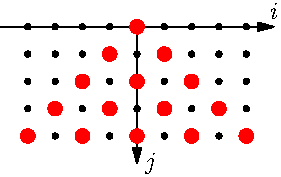
\includegraphics{./Eboustro_1_fig.pdf}
  \caption{Partie $\mathcal{E}$.}
  \label{fig:Eboustro_1}
\end{figure}

\begin{figure}
  \centering
  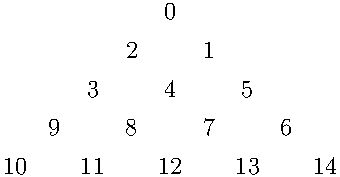
\includegraphics{./Eboustro_2_fig.pdf}
  \caption{Numérotation et ordre}
  \label{fig:Eboustro_2}
\end{figure}
On associe à chaque point de $\mathcal{E}$ un nombre que l'on forme par un procédé analogue à celui du triangle de Pascal avec les règles suivantes (voir figure \ref{fig:Eboustro_3}) .
\begin{itemize}
  \item Le nombre $1$ est associé au point $(0,0)$ de numéro $0$.
  \item Les lignes sont parcourues alternativement d'un côté à  l'autre. Le premier élément d'une nouvelle ligne reçoit toujours $0$.
  \item Le nombre associé à un point d'une ligne est la somme des nombres associés au point précédent et au point de la ligne du dessus.
\end{itemize}
\begin{figure}
  \centering
  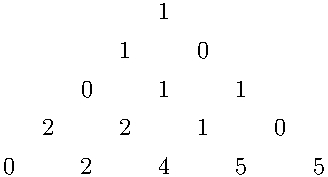
\includegraphics{./Eboustro_3_fig.pdf}
  \caption{Nombres associés aux points de $\mathcal{E}$.}
  \label{fig:Eboustro_3}
\end{figure}
\begin{enumerate}
  \item Soit $(i,j)\in \Z \times \N$. Caractériser par des propriétés de $i+j$ et $i-j$ le fait que $(i,j)\in \mathcal{E}$.
  \item Calculer mathématiquement le numéro d'un point $(i,j)\in \mathcal{E}$.
  \item Former une fonction nommée \verb|suivant| qui prend deux paramètres \verb|i| et \verb|j| désignant respectivement des éléments $i$ de $\Z$ et  $j$ de $\N$ tels que $(i,j)\in \mathcal{E}$ et qui renvoie le tuple des deux coordonnées du point suivant de $\mathcal{E}$ pour l'ordre choisi.
  \item Former une fonction nommée \verb|num| qui prend deux paramètres \verb|i| et \verb|j| désignant respectivement des éléments $i$ de $\Z$ et  $j$ de $\N$ et qui renvoie le numéro du point $(i,j)$ s'il appartient à $\mathcal{E}$ et $-1$ s'il n'y appartient pas. Cette fonction devra utiliser la fonction \verb|suivant| et non l'expression mathématique.
  \item Former une fonction nommée \verb|boustro2| qui prend un paramètre \verb|n| désignant un entier naturel $n$ et qui renvoie un dictionnaire (indexé par les tuples de coordonnées) des valeurs associées aux $n$ premiers points de $\mathcal{E}$. On pourra utiliser une liste contenant les deux coordonnées d'un point ainsi que le sens de parcours (codé par $+1$ pour gauche-droite et $-1$ pour droite-gauche) au point représenté. 
\end{enumerate}

\end{enumerate}
